\documentclass[10pt]{article}
\usepackage[T1]{fontenc}
%\usepackage[utf8]{inputenc}
\usepackage[french]{babel}
\usepackage{graphics}
\title{Page de garde du TER et du M\'emoire de l'Universit\'e des Antilles-Guyane}
\newcommand{\LOL}[1]{\mbox{\raisebox{1em}{\rotatebox{-90}{:-)}}\raisebox{2em}{\rotatebox{-90}{:-)}}\hspace{-2ex}\rotatebox{-90}{:-)}}~#1~%
\mbox{\raisebox{2em}{\rotatebox{-90}{:-)}}\hspace{-2ex}\rotatebox{-90}{:-)}\raisebox{1em}{\rotatebox{-90}{:-)}}}}

\usepackage[pdftex,colorlinks]{hyperref}
\hypersetup{%
   pdfauthor=C\'edrick \textsc{Copol},%
   pdftitle=Page de garde du TER et du M\'emoire de l'Universit\'e des Antilles-Guyane%
}

\author{C\'edrick \textsc{Copol}}

\begin{document}
\maketitle
\tableofcontents

\section{Contenu }
Pour faire la page de garde vous trouverez les fichiers suivants :

\begin{itemize}
 \item	PagedegardeUAG-doc.pdf \og la documentation que vous lisez en ce moment \fg{}
 \item	nouveau\_logo\_uag.eps
 \item	nouveau\_logo\_uag.png
 \item	pagedegardeUAG.sty
\end{itemize}

\section{Mode d'emploi }

\begin{enumerate}
 \item  Placez dans votre dossier de travail, celui contenant votre .tex, le dossier uag\_style

 \item  Editez votre .tex

  \item Pr\'eciser au besoin a4paper , dans \textbackslash documentclass[a4paper]\{\ldots\}

 \item  Pour charger l'extention \emph{pagedegardeUAG} taper dans le pr\'eambule
\mbox{\textbackslash usepackage[X]\{uag\_style/pagedegardeUAG\}}
	o\`u X prend l'une de ces 3 valeurs en fonction de ce que vous pr\'eparer \LOL{bien-sur}:
		\begin{itemize}
		    \item \textbf{ter};
		    \item \textbf{memoire};
		    \item \textbf{rapport}.
		\end{itemize}

Quoi de plus parlant qu'un exemple ? \LOL{RIEN}

	    Vous pr\'eparez un \og ter \fg{} alors mettez 
	\mbox{\textbackslash usepackage[ter]\{pagedegardeUAG\}}.

	    Vous pr\'eparez un \og memoire \fg{} alors mettez 
	\mbox{\textbackslash usepackage[memoire]\{pagedegardeUAG\}}.

	Les classes support\'ees pour l'instant sont :
	\begin{itemize}
		\item article
		\item report
		\item book
	\end{itemize}
		(pour les autres il ne vous reste qu'\`a \LOL{essayer} )

 \item  Mettez dans le pr\'eambule 
	\begin{itemize}
		\item \mbox{\textbackslash usepackage\{xcolor\}}
		\item \mbox{\textbackslash usepackage\{graphicx\}}
	\end{itemize}
 \item  Et enfin renseignez les commandes suivantes :
	\begin{itemize}
		\item \mbox{\textbackslash title\{ \}}
		\item \mbox{\textbackslash author\{Pr\'enom\}\{Nom\}\{votreadress@trucmuche.chose\}}
		\item \mbox{\textbackslash annee\{2008-2009\}}
		\item \mbox{\textbackslash Encadrant\{Mme, Mlle, M. Prof encadrant\}}
	\end{itemize}

 \item  Mettre la commande \mbox{\textbackslash maketitle} apr\`es \mbox{\textbackslash begin\{document\}}.

 \item  Attention pour obtenir le r\'esultat attendu vous devez compiler avec \LaTeX{} puis dvips puis ps2pdf (ou pstopdf).
       \LOL{Comment faire ?} Cherchez dans votre \'editeur de texte pr\'ef\'er\'e d\'edi\'e \`a \LaTeX, il s'aura le faire. 

 \item  Bonne journ\'ee en esp\'erant que sa fonctionne.
   Je vous remercie d'utiliser mon extension et bien-sur :
			BONNE CHANCE !!
\end{enumerate}

\section{Les commandes}

\begin{tabular}{|p{2.5cm}|p{9cm}|}
\hline
  \bf \textbackslash Imawoman \textbackslash Imaman & Renseigner votre sexe. Le but est de mettre
  \textbf{Pr\'esent\'e}, ou \textbf{Pr\'esent\'ee}. Si ni aucune de ces commandes n'est mise alors on pourra lire
  \textbf{Pr\'esent\'e(e)}.\\\hline
  \bf \textbackslash title     & Pour le titre\\\hline
  \bf \textbackslash author    & \textbf{ \textbackslash author}\{Pr\'enom\}\{Nom\}\{courriel\} \\\hline
  \bf \textbackslash Encadrant & \textbf{ \textbackslash Encadrant}\{Pr\'enom\}\{Nom\}\{Profession\} \\\hline
\end{tabular}

\section{R\'esolution de probl\`eme}
\subsection{Windows mon cher windows}

	Cette section ne concerne que les utilisateur de Windows (peut-\^etre Mac mais je n'avais personne pour tester). Alors les autres passez votre chemin.
	Il faut indiquer a MiK\TeX{} qu'il doit utiliser un format A4 mais un vrai format A4.
	Pour cela suivez le guide:

Cliquez sur le menu D\'emarrer puis sur \og tous les programmes\fg{}. Cherchez MiK\TeX{} 2.7(ou une autre version), un menu d\'eroulant s'ouvre avec ceci Browse Packages, 
Previewer, Settings et Update. Cliquez sur \og Settings \fg{} la fen\^etre \ref{image} s'ouvre :


\begin{figure}%[h]
\hspace*{-2cm}  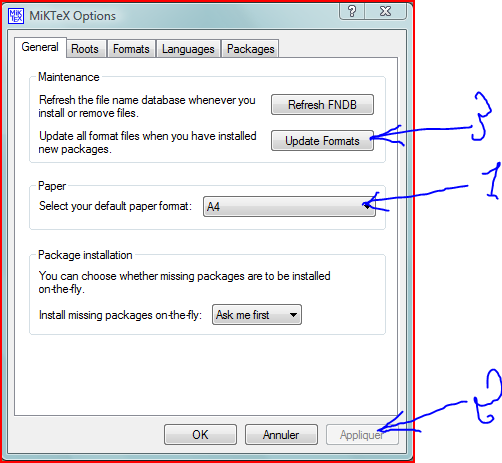
\includegraphics{miktex_option.png}
\caption{MiKTEX Settings}\label{image}
\end{figure}
\begin{description}
 \item[\'Etape 1] choisir A4 et non A4(size)
 \item[\'Etape 2] cliquez sur Appliquer
 \item[\'Etape 3] cliquez sur Update formats
 \end{description}



\subsection{Probl\`emes possibles}

Cette section est  relative aux probl\`emes rencontr\'ees avec l'ancienne version (celle d'avril 2009) il est possible
 que ces probl\`emes aient disparus.\\
	Le cadre bleu n'est pas adjacent au bord droit de la feuille

\begin{itemize}
 \item  enlever l'option twoside dans \textbackslash documentclass.
 \item probl\`eme du aux extensions \emph{geometry}, \emph{fullpage} enlever les s'il ne sont pas utilis\'es.
 \item  Il peut \^etre n\'ecessaire d'\'ecrire\\ 
			\mbox{\textbackslash usepackage\{amsmath,amsfonts,amssymb,amsthm\}}
		 au lieu de \mbox{\textbackslash usepackage\{amsmath\}} \mbox{\textbackslash usepackage\{amsfonts\}} \mbox{\textbackslash usepackage\{amssymb\}} \mbox{\textbackslash usepackage\{amsthm\}}.
\end{itemize}

Si malgr\'e mes explications rien ne marche modifier directement le fichier main.tex .
Ainsi vous aurez un fichier ne contenant que la page de garde et un autre contenant votre travail, ou compiler chez un ami pour qui cela fonctionne.
\noindent
\begin{tabular}{lp{5cm}}
\hline
  Le d\'ebut du mot M\'emoire ou Travaux est rogn\'e&%
   Vous avez oubli\'e de mettre l'option a4paper a documentclass.
   exple : \textbackslash documentclass[a4paper]\{article\}
   Si \c ca ne fonctionne pas et que vous utilis\'ee MikTeX voir plus haut.
\end{tabular}

% Le début du mot Mémoire ou Travaux est rogné,
   

Prendre en main la page de garde

Vous avez la possibilité de modifier le position du filigrane de manière aisée.
Il suffit pour cela de redéfinir certaines commandes.
    \textbackslash nameXpos et/ou \textbackslash nameYpos
name peut être 'entete', 'Filigrane' 

\end{document}
